\chapter{Analýza implementace knihovny GTTG}
Text této kapitoly podrobně analyzuje možné přístupy k~implementaci částí knihovny GTTG, aby byly splněny cíle \ref{uvod:cil:knihovna} \ref{uvod:cil:knihovna:ruzne_typy_njr} - \ref{uvod:cil:knihovna:dotnet_standard} uvedené na konci kapitoly \ref{kap:uvod} a~požadavky \ref{spec:req:interaction_trans1} - \ref{spec:zobrazitelne_prvky_vykresleni} uvedené v~kapitole \ref{kap:spec}.

\section[Implementace komponenty a~prostředí pro kreslení]{Implementace komponenty a~prostředí pro kreslení}
\label{kap:impl:komp}
Jedním z~cílů pro vývoj knihovny je zajistit její integrovatelnost do aplikací ~(cíl \textbf{\color{goalcolor}G1}\ref{uvod:cil:knihovna:integrace_do_aplikaci}). Toho dosáhneme pomocí správné implementace komponenty. Jelikož knihovna SkiaSharp bude při určování implementace komponenty a~integrace knihovny do aplikací hrát zásadní roli, nejdříve se před samotným rozborem implementace seznámíme s~jejími základními principy fungování.

\subsection{Úvod do práce s~knihovnou SkiaSharp} 
Základem pro kreslení v~knihovně SkiaSharp je třída \texttt{SKCanvas}, která představuje plátno pro kreslení. Mezi instanční metody této třídy patří kreslící příkazy (například \texttt{DrawText()}, \texttt{DrawCircle()}), které se na základě dodaných parametrů nanáší na plátno. Jelikož je knihovna SkiaSharp 2D, pořadí nanášení příkazů na plátno je určeno pořadím volání metod. Kreslení na plátno, vzniklé jako výsledek aplikování několika kreslících příkazů na následujícím fragmentu kódu, je uvedeno na obrázku \ref{fig:skia_kresleni_ukazka}.

\begin{csharpcode}
var paint = new SKPaint {Color = SKColors.Green, Style = SKPaintStyle.Fill};
canvas.DrawRect(SKRect.Create(x: 145, y: 10, width: 75, height: 30), paint);
paint.Color = SKColors.BlueViolet;
canvas.DrawCircle(new SKPoint(x: 70, y: 70), radius: 25, paint: paint);
\end{csharpcode}

\begin{figure}[!hbt]
	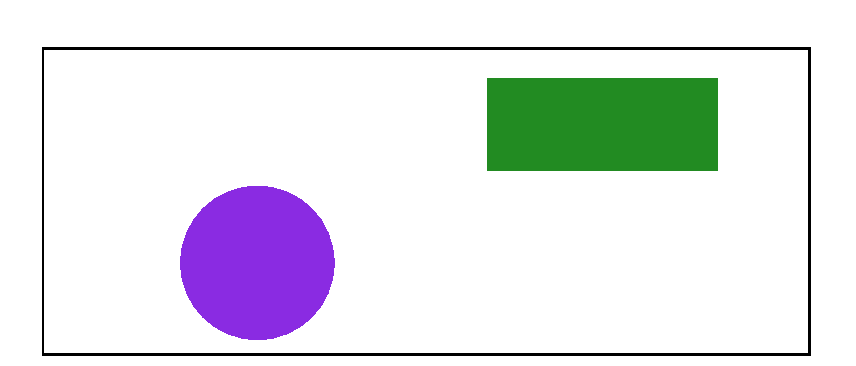
\includegraphics[width=\textwidth]{../img/kap3_skia_matrix_identity}
	\caption{Kreslení na plátno odpovídající kreslícím příkazům v~předchozím fragmentu kódu}
	\label{fig:skia_kresleni_ukazka}
\end{figure}

\subsubsection*{Transformace kreslících příkazů}
\label{kap3:skia_intro_transformations}
Plátno \texttt{SKCanvas} je možné konfigurovat přenastavením matice označované jako \texttt{transform matrix} a~výřezu plátna, který se nazývá \texttt{clip}. Část kreslícího příkazu, který se nachází mimo \texttt{clip}, se nevykreslí. Nastavení \texttt{transform matrix} ovlivňuje výsledek kreslících příkazů. Na obrázku \ref{fig:skia_kresleni_ukazka_transformace} se na plátno aplikovaly stejné příkazy jako při kreslení na obrázku \ref{fig:skia_kresleni_ukazka}, pouze se před jejich aplikací nastavila \texttt{transform matrix} na následujícím fragmentu kódu. Obsah výkresu je nyní transformován rotací o~$\pi$/8 po směru hodinových ručiček se středem v~levém horním rohu zeleného obdélníku.

\begin{csharpcode}
var pivotX = 145; var pivotY = 10;
SKMatrix.Rotate(ref matrix, (float) Math.PI / 8, pivotX, pivotY);
canvas.SetMatrix(matrix);
\end{csharpcode}

\begin{figure}[!hbt]
	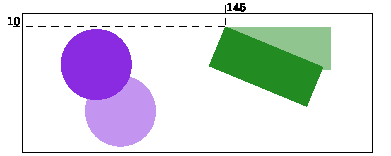
\includegraphics[width=\textwidth]{../img/kap3_skia_matrix_translate_scale}
	\caption{Výkres \ref{fig:skia_kresleni_ukazka} se změněnou \texttt{transform matrix}. Původní výkres je pro porovnání uveden ve stínu}
	\label{fig:skia_kresleni_ukazka_transformace}
\end{figure}

Konfigurace \texttt{transform matrix} se vykonává voláním \texttt{SetMatrix()}, \texttt{clip} se aplikuje vzhledem k~současné \texttt{transform matrix} například pomocí \texttt{ClipRect()}. \texttt{Transform matrix} i~\texttt{clip} je možné efektivně měnit a~vracet do původních stavů, jelikož konfigurace jsou plátnem ukládány na jeho zásobník modifikací. Pro každou sérii kreslících příkazů je tak možné použít jinou transformaci.

\subsubsection*{Sestrojení plátna}
Pokaždé, když chceme pracovat s~knihovnou SkiaSharp, musíme pro kreslení získat instanci plátna \texttt{SKCanvas}. Plátno může být sestrojeno nad existující bitmapou nebo může být vytvořeno jako instanční proměnná třídy \texttt{SKSurface}, která je zodpovědná za práci s~nástrojem poskytující pixely, na které \texttt{SKCanvas} kreslí. Je tak možné rozhodnout, jestli jsou pixely alokovány v~paměti nebo GPU. Dále je možné, aby SkiaSharp vykreslovala obsah plátna do PDF nebo jako vektorovou grafiku v~SVG. Jednou z~vlastností \texttt{SKCanvas} i~\texttt{SKSurface} je, že po vytvoření již nemůžou měnit svou velikost.

\newpage
\subsubsection*{Podpora v~rámci uživatelských rozhraní}
\label{kap3:skia_ui_elements}
Knihovna SkiaSharp nabízí pro některé GUI frameworky implementaci prvku uživatelského rozhraní, jehož plocha se používá jako plátno \texttt{SKCanvas}.
To přináší vývojářům zásadní ulehčení jejich práce, jelikož prvek sám sestrojí \texttt{SKSurface} a~při změně velikosti prvku vytvoří nový s~upravenou velikostí. Kdykoliv, když je vizualizace prvku invalidována, je obnoven kreslící cyklus, v~kterém vývojář pracuje s~plochou prvku uživatelského rozhraní jako s~\texttt{SKCanvas}. Vývojáři díky těmto implementacím nemusí pracovat s~kreslícím \textit{backendem}, který by museli zapojit do \texttt{SKSurface} za poskytnutí mnoha parametrů popisující jeho nastavení.

\subsection{Integrace knihovny do aplikací}
Na základě zmíněných vlastností knihovny SkiaSharp si nyní popíšeme, jak naše knihovna bude integrována do aplikací. V~rámci této integrace je nutné určit, jaké nástroje musí vývojář knihovně dodat.

\subsubsection*{Reprezentace jednotek pixelů}
\label{kap3:jednotky_pixelu}
V~rámci implementace komponenty můžeme splnit požadavky \ref{spec:req:unit1} a~\ref{spec:req:unit2} související s~existencí plátna v~různých jednotkách pixelů. Uvedli jsme si, že \linebreak SkiaSharp nabízí implementaci UI prvků určených pro kreslení. U~těchto prvků je možné nastavit jednotky pixelů plátna \texttt{SKCanvas}. V~prvku \texttt{SKElement} GUI frameworku WPF se jednotky pixelů nastavují vlastností \texttt{IgnorePixelScaling} uvedené na následujícím fragmentu kódu.

\begin{csharpcode}
public class SKElement : FrameworkElement {

/// <summary>
/// Gets or sets a~value indicating whether the drawing canvas
/// should be resized on high resolution displays.
/// </summary>
/// <remarks>
/// By default, when false, the canvas is resized to 1 canvas
/// pixel per display pixel. When true, the canvas is resized to device
/// independent pixels, and then stretched to fill the view. Although
/// performance is improved and all objects are the same size on different
/// display densities, blurring and pixelation may occur.
/// </remarks>  
public bool IgnorePixelScaling {
\end{csharpcode}

Komentář vysvětluje, že pokud pixely plátna \texttt{SKCanvas} odpovídají pixelům nezávislých na zařízení, je dodána \texttt{SKSurface} bitmapa v~jednotkách pixelů s~DPI 96, které odpovídá ve WPF jednotkám pixelů nezávislých na zařízení. Bitmapa pak pro každý takový pixel může v~závislosti na zařízení použít několik fyzických pixelů.

Pokud bychom řešili tento problém obecně, plátno by bylo vytvořeno ve velikosti odpovídající ploše prvku v~jednotkách pixelů zařízení a~více pixelů zařízení by mohlo odpovídat jednomu pixelu nastavením škálování v~\texttt{transform matrix} plátna. Pokud bychom velikost komponenty určovali pomocí velikosti plátna \texttt{SKCanvas}, nastala by tímto způsobem nekonzistence v~reprezentaci velikostí -- v~případě nastavení \texttt{IgnorePixelScaling} je plátno udáváno v~konečné velikosti pixelů nezávislých na zařízení a~v~případě nyní zmiňovaného způsobu by odpovídalo velikosti pixelů zařízení, ačkoliv v~obou případech chceme v~komponentě pracovat s~jednotkami pixelů nezávislých na zařízení. I~přes tyto nevýhody bychom chtěli takovou konfiguraci umožnit. 

Rozhodli jsme se proto, že velikost komponenty bude explicitně uváděna jiným způsobem a~s~velikostí \texttt{SKCanvas} knihovna pracovat nebude. Vývojář, který bude chtít použít zvětšování pomocí \texttt{transform matrix}, sám matici nastaví a~knihovna mu tuto konfiguraci nezmění. Protože existují různé způsoby, jak můžou být pro \texttt{SKSurface} alokovány pixely, nechceme v~knihovně vytvářet nové plátno v~bitmapě a~budeme po vývojáři požadovat, aby dodal vlastní \texttt{SKSurface} \linebreak s~\texttt{SKCanvas}. Jiná implementace by byla neefektivní vzhledem k~možnostem\linebreak knihovny SkiaSharp. Zároveň požadujeme, aby vývojář provedl všechna doposud popisovaná nastavení sám mimo knihovnu. Pokud se komponentě předávají body z~plochy prvku, která pracuje s~jinými jednotkami pixelů, vývojář musí převod jednotek sám implementovat. Jelikož už vývojář v~této konfiguraci pracuje s~hodnotou DPI, která je uvedena v~požadavku \ref{spec:req:unit2}, hodnotu DPI komponentě nastaví sám. Všechny tyto konfigurace se tak odehrávají na stejné úrovni a~knihovna bude konzistentně pracovat se stejnými jednotkami velikosti.

\subsection{Reprezentace časových intervalů}
Musíme najít způsob, jak reprezentovat časové intervaly definované \ref{spec:req:int1} a~\ref{spec:req:int2}. Zároveň \ref{spec:req:conv1} požadujeme, aby bylo možné časové údaje používané v~reprezentaci intervalů převádět do bodů plátna. Převod by měl být co nejméně komplikovaný. Doposud jsme si uváděli situace, kdy časový interval nepřesáhne několik hodin a~proto by se nabízelo použít k~reprezentaci časových údajů struktury, které reprezentují pouze čas, ale neobsahují už informaci o~datu. Každá aplikace ale pracuje s~jinou reprezentací časových údajů v~jejím modelu dat. Existují aplikace, které sledují současný provoz a~v~časových údajích zahrnují i~datum.

K~reprezentaci časových údajů v~knihovně jsme se proto rozhodli použít strukturu \texttt{DateTime}. Převod jiných struktur pracujících s~časovými údaji do hodnot \texttt{DateTime} není komplikovaný a~převod v~rámci \ref{spec:req:conv1} je přímočarý -- rozdíl konce a~začátku intervalu vytvoří strukturu \texttt{TimeSpan} obsahující hodnotu \texttt{TotalMilliseconds}, s~jejíž násobky jde dále při převodu pracovat. Při použití data i~času nemůže docházet k~nejednoznačnostem při porovnávání a~převodu časových intervalů.

\subsection{Modifikace komponenty}
\label{kap3:modifikace_komponenty}
Modifikace komponenty jako translace nebo škálování nesmí překročit ohraničení definované \ref{spec:req:interaction_trans1}. Jelikož se chybné modifikace mohou při interakci uživatele s~komponentou vyskytovat běžně, nechceme, aby vyhazovaly výjimky. Zároveň ale chceme vývojáře informovat o~úspěšnosti modifikace, jelikož na jejím provedení může být například závislé vykreslení obsahu a~nechceme zbytečně vykreslovat modifikací nezměněný obsah. Rozhodli jsme se, že každé volání modifikace bude mít jako návratovou hodnotu výčtový typ, který bude poskytovat informace o~úspěšnosti modifikace. Na následujícím fragmentu kódu je příklad takového výčtového typu pro modifikaci \ref{spec:req:interaction_zoom1} škálující zobrazení:

\begin{csharpcode}

public enum ScaleTransformationResult {
    ViewModifiedWithTransformedOrigin,
    ViewModifiedWithSameOrigin,
    ViewUnmodified
}

public ScaleTransformationResult TryScale(SKPoint origin, float delta) {
	/*...*/
}
\end{csharpcode}

Pro případ, kdy nastane stav \ref{spec:req:interaction_zoom2} a~pohled by se vyskytl mimo ohraničení \ref{spec:req:interaction_trans1}, je vrácen \texttt{ViewModifiedWithTransformedOrigin}. Rozhodli jsme se, že se pohled v~rámci volání \texttt{TryScale()} deterministicky upraví tak, aby byl posunut o~délku, kterou v~ohraničení překračuje. V~případě, že faktor škálování je menší než jedna, je vrácen \texttt{ViewUnmodified}.

\subsubsection*{Práce s~komponentou ve vícevláknovém prostředí}
Může docházet k~případům, kdy vývojář bude ke knihovně přistupovat z~více vláken. Například je v~rámci aplikace spuštěn periodický časovač, který běží v~dalším vlákně a~opakovaně upravuje nějakou část komponenty, aby odpovídala modelu dat v~aplikaci. Pokud by se taková změna stavu komponenty z~jiného vlákna vyskytla během vykreslování nebo jiných změn v~komponentě, může se vyskytnout chybový stav označovaný jako \textit{race condition}. Chceme určit postup, jak systematicky těmto problémům předcházet. Jelikož knihovna bude obvykle součástí uživatelských rozhraní, která řeší podobné problémy pro jejich prvky, nabízí se jejich řešení rozšířit i~na naší knihovnu. Každé uživatelské rozhraní definuje svá pravidla pro práci ve vícevláknovém prostředí označovaná jako \textit{threading model}. Většinou je pravidlem povolovat u~každého prvku změnu jeho stavu pouze z~vlákna, které se nazývá \textit{UI vlákno}. Kdykoliv uživatel změní stav prvku z~jiného vlákna, je vyhozena výjimka. Práci z~jiného vlákna modifikující stav prvku je však možné zařadit do UI vlákna přes strukturu obecně nazývanou \textit{dispatcher}. Takto je řešena synchronizace na úrovni prvků uživatelského rozhraní. Například v~GUI frameworku WPF je každý UI prvek potomkem abstraktní třídy \texttt{DispatcherObject}, která nabízí nástroje pro ověření přístupu přes metody uvedené na následujícím fragmentu kódu. Při nastavování vlastností prvků uživatelského rozhraní se pak kontroluje přístup v~rámci volání \texttt{SetValue()} a~metody přístup kontrolují přes \texttt{VerifyAccess()}.

\begin{csharpcode}
public abstract class DispatcherObject {

	public void VerifyAccess() {
      this._dispatcher?.VerifyAccess();
    }

	public void SetValue(DependencyProperty dp, object value) {
      this.VerifyAccess();
\end{csharpcode}

Pokud bychom se rozhodli řešit tento problém na úrovni knihovny, museli bychom najít řešení, které bude jednoduché na implementaci a~zajistí konzistentní chování při práci s~celým obsahem knihovny. Nemůžeme převzít žádné konkrétní řešení, které existuje v~rámci nějakého GUI frameworku, jelikož jedním z~cílů je zajistit přenositelnost knihovny na úrovni .NET Standard (cíl \textbf{\color{goalcolor}G1}\ref{uvod:cil:knihovna:dotnet_standard}). Mohli bychom implementovat vlastní řešení, které by se chovalo podobně jako zmíněný \texttt{DispatcherObject} a~dispatcher, ale zajistit jeho správnost i~udržitelnost by bylo náročné. Nalezením řešení na úrovni knihovny bychom také způsobili zpomalení aplikací, které budou ke kódu knihovny přistupovat z~jednoho vlákna. Z~těchto důvodů jsme se rozhodli, aby vývojář řešil problémy synchronizace na úrovni uživatelského rozhraní s~nástroji, které GUI frameworky nabízí. Následující fragment kódu z~vlákna běžícího vedle UI vlákna v~aplikaci ve WPF zařadí do UI vlákna přes \texttt{Dispatcher.Invoke()}  vykonání lambda funkce, která přidá nový vlak do modelu vykreslovaného komponentou.

\begin{csharpcode}
Train newTrain = /*...*/;

Dispatcher.Invoke(() => {
	Model.Trains.Add(newTrain);
});
\end{csharpcode}

\subsection{Reprezentace plátna v~knihovně}
\label{fig:analyza_impl:platno}
Podle požadavku \ref{spec:req:canvas1} chceme vývojářům poskytnout plátno nákresného jízdního řádu, které má být nastaveno tak, aby v~komponentě byl zobrazen jeho výřez v~závislosti na jejím stavu. Toto plátno nazveme \texttt{ContentCanvas}. Implementaci jeho nastavení v~komponentě se nyní budeme věnovat.

Pro vykreslení správného výřezu plátna \texttt{ContentCanvas} můžeme nastavit \texttt{transform matrix} na plátně \texttt{SKCanvas}, které podle \ref{kap3:jednotky_pixelu} knihovně dodává vývojář k~vykreslení. V~počátečním stavu zobrazeném na obrázku \ref{fig:impl:platno_matice_identity} je \texttt{transform matrix} identita. Modifikace komponenty popsaná \ref{spec:req:interaction_trans2} odpovídá operaci translace, \ref{spec:req:interaction_zoom1} odpovídá škálování. Upravená \texttt{transform matrix} po modifikaci posunem je zobrazena na obrázku \ref{fig:impl:platno_matice_transformace}. Bod [300,300] na \texttt{ContentCanvas} se nyní mapuje na [0,0] a~vykreslí se na levém horním rohu komponenty. 

\begin{figure}[h]
\centering
\begin{subfigure}{0.45\textwidth}
	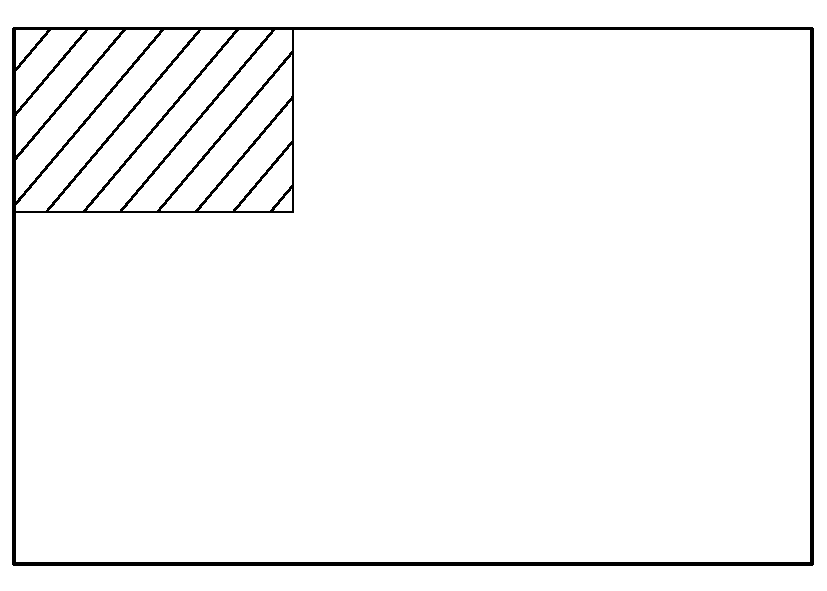
\includegraphics[width=\linewidth]{../img/kap3_komponenta_identita}
	\centering

$\begin{pmatrix}
1 & 0 & 0 \\
0 & 1 & 0 \\
0 & 0 & 1
\end{pmatrix}$

	\caption{Identita}
	\label{fig:impl:platno_matice_identity}
\end{subfigure}
\begin{subfigure}{0.45\textwidth}
	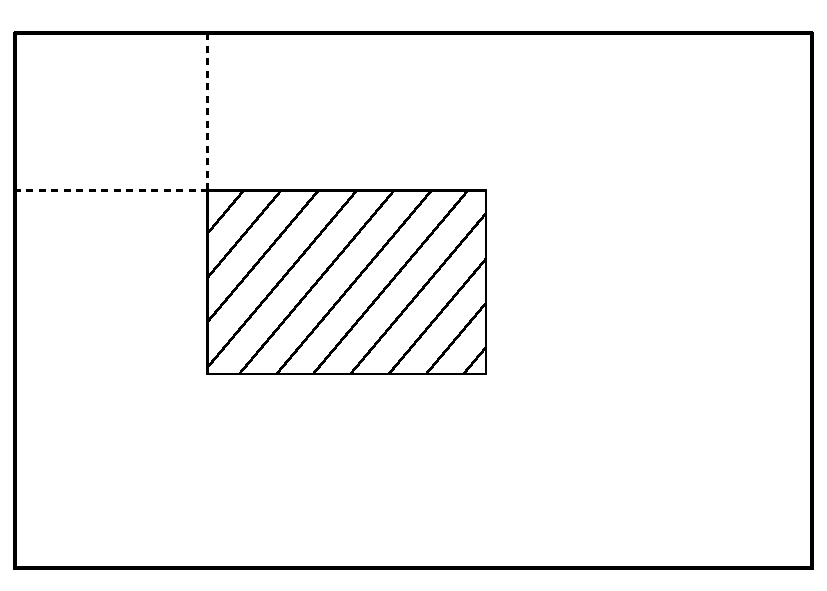
\includegraphics[width=\linewidth]{../img/kap3_komponenta_translace}
\centering
$\begin{pmatrix}
1 & 0 & 0 \\
0 & 1 & 0 \\
-300 & - 300 & 1
\end{pmatrix}$

	\caption{Translace}
	\label{fig:impl:platno_matice_transformace}
\end{subfigure}
\end{figure}

\newpage
Nastavení \texttt{transform matrix} plátnu \texttt{SKCanvas} pomocí \texttt{SetMatrix()} se \linebreak v~knihovně Skia v~tomto případě optimalizuje -- její implementace je schopna zjistit, že nastavovaná matice odpovídá matici posunu a~při následujícím aplikování kreslících příkazů neproběhne obecná transformace násobením s~nastavenou maticí, ale pouze se k~bodům kreslícího příkazu přičte po osách délka posunu. Protože jiná implementace by byla neefektivní vzhledem k~možnostem knihovny Skia, rozhodli jsme se výřez nastavit tímto způsobem.

\subsubsection*{Vykreslování obsahu mimo zobrazovanou oblast v~komponentě}
\label{kap3:view_element_bounding_check}
Ve dvou bodech si uveďme, jaké výhody pro vývojáře knihovny přináší používání plátna \texttt{ContentCanvas}:

\begin{enumerate}
	\item \label{impl:njr_platno_vyhody_kresleni} Pro vývojáře se oddělil proces zobrazení obsahu komponenty od vykreslení obsahu nákresného jízdního řádu. Díky používání \texttt{ContentCanvas} vývojář nemusí počítat, jaký jeho výřez se v~komponentě zobrazí a~může vykreslit celý obsah nezávisle na tomto zobrazení.
	\item \label{impl:njr_platno_vyhody_rozmisteni} Výpočet, v~němž se rozmístí obsah zobrazený v~komponentě a~který jsme nazvali \textit{cyklem rozmístění}, probíhá pro celý obsah plátna \texttt{ContentCanvas}. Cyklus rozmístění musí probíhat v~případě změny velikosti komponenty. Modifikace měnící zobrazovaný výřez v~komponentě s~cyklem rozmístění nesouvisí.
\end{enumerate}

Používání plátna \texttt{ContentCanvas} může vedle těchto výhod představovat výkonnostní problém. Na obrázku \ref{fig:platno_mimo_komponentu} se nachází šedě podbarvená část jeho obsahu, která se v~komponentě nezobrazí a~přesto se vykresluje. Ušetřený čas za nehledání zobrazovaného obsahu tak může být převážen vykonáním kreslících příkazů, které se nezobrazí.

\begin{figure}[!bht]
	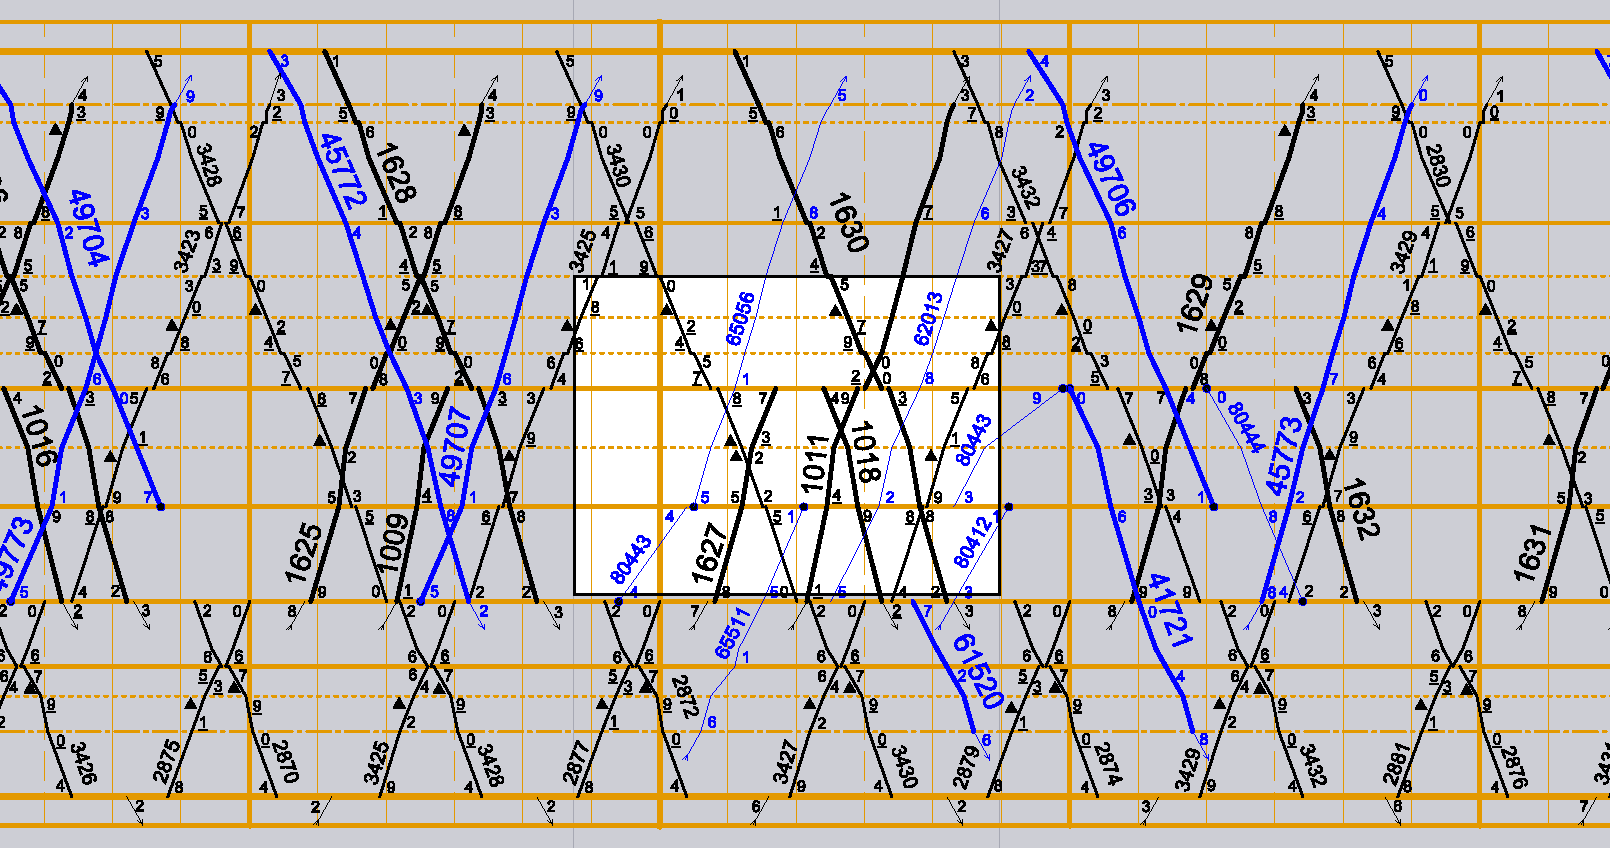
\includegraphics[width=\textwidth]{../img/kap3_platno_mimo_komponentu}
	\caption{Šedě podbarvený obsah \texttt{ContentCanvas} nacházející se mimo zobrazení komponenty}
	\label{fig:platno_mimo_komponentu}
\end{figure}

Hledání zobrazovaného obsahu budeme místo vývojáře řešit na úrovni \linebreak knihovny efektivní metodou, která je založena na následujícím pozorování. Podívejme se, na jaký obsah \texttt{ContentCanvas} se používá nejvíce kreslících příkazů. Souřadnicová síť jako několik čar nepředstavuje pro kreslení zásadní problém, stejně tak i~lomené čáry znázorňující průběh jízdy vlaků. Ke každému vlaku ale existuje několik zobrazitelných prvků, které často obsahují pro kreslení složitý obsah, jakým je například text. Na obrázku \ref{fig:prvky_mimo_komponentu} jsme v~části obsahu, která se v~komponentě nezobrazí, ohraničili zobrazitelné prvky červenými obdélníky.

\begin{figure}[!hbt]
	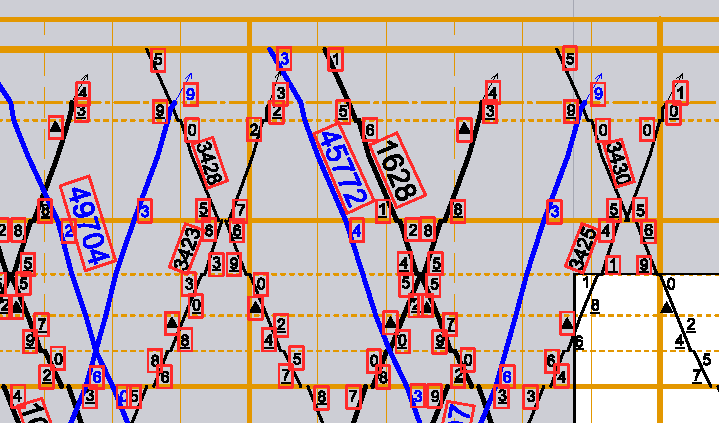
\includegraphics[width=\textwidth]{../img/kap3_zobrazitelne_prvky_mimo_komponentu}
	\caption{Zobrazitelné prvky označené červenými obdélníky se nacházejí mimo zobrazení komponenty}
	\label{fig:prvky_mimo_komponentu}
\end{figure}

Toto pozorování nyní spojíme s~prací se zobrazitelnými prvky v~rámci cyklu rozmístění. Strategie, které jsme si představili v~\ref{kap:spec:obsah_njr}, v~cyklu rozmístění pracují se zobrazitelnými prvky jako s~obdélníky, které někam umístí a~transformacemi rotací a~škálování je upraví. Tyto obdélníky odpovídají červeným obdélníkům na obrázku \ref{fig:prvky_mimo_komponentu}. Jelikož probíhá cyklus rozmístění na celém obsahu, jsou všechny zobrazitelné prvky před vykreslením již rozmístěny a~obdélníky je tak možné určit. Zobrazitelný prvek vykreslíme pouze v~případě, pokud se část jeho obdélníku nachází v~komponentě.

Nalezli jsme řešení, které je založeno na existující implementaci knihovny a~vzniká jako vedlejší výsledek rozmístění zobrazitelných prvků v~cyklu rozmístění. Kreslení obsahu tak zabere méně času než v~případě, kdy se vykreslí celý obsah nebo když by vývojář používal své vlastní řešení pro hledání zobrazeného obsahu v~komponentě.
\newpage
\section{Práce s~obsahem nákresného jízdního řádu}
V~této části určíme, jak implementovat knihovnu tak, aby umožnila tvorbu různých typů nákresných jízdních řádů (cíl \textbf{\color{goalcolor}G1}\ref{uvod:cil:knihovna:ruzne_typy_njr}) a~byly splněny požadavky kapitoly \ref{kap:spec}, které souvisí s~prací s~obsahem nákresného jízdního řádu.

\subsection{Implementace zobrazitelných prvků}
\label{kap3:zobrazitelne_prvky}
Zobrazitelným prvkům chceme v~cyklu rozmístění podle \ref{spec:zobrazitelne_prvky2} přidělovat různými způsoby jejich velikost. S~velikostí a~umístěním prvku pracují požadavky \textit{hit-testování} \ref{spec:req:hit-test1}, vykreslování \ref{spec:zobrazitelne_prvky_vykresleni} a~umístění do strategií \ref{spec:req:strategie2}. Před zvážením možné implementace cyklu rozmístění prvků určíme, jak na ní bude závislá implementace těchto požadavků.

\subsubsection*{Vykreslení zobrazitelných prvků}
\label{kap3:vykresleni_zobrazitelnych_prvku}
Pro vykreslování zobrazitelných prvků chceme vývojářům podle \ref{spec:zobrazitelne_prvky_vykresleni} předávat vlastní plátno, které bude odpovídat velikost prvku. V~podkapitole \ref{kap3:jednotky_pixelu} jsme se rozhodli, že knihovna bude pracovat pouze s~jedním plátnem -- \texttt{SKCanvas} poskytnutým vývojářem. Plátno pro zobrazitelný prvek tak bude představovat vytvoření pohledu na toto plátno, podobně jako \texttt{ContentCanvas}, jehož pohled jsme nastavili pomocí \texttt{transform matrix}. Na základě výhod uvedených v~\ref{fig:analyza_impl:platno} jsme se také rozhodli pro vykreslení plátna zobrazitelných prvků nastavit \texttt{transform matrix}. Hodnoty této matice budou závislé na umístění prvku na \texttt{ContentCanvas} a~\texttt{transform matrix} plátna \texttt{ContentCanvas}. Umístění prvku budeme reprezentovat maticí, kterou nazveme \texttt{placement matrix} a~abychom získali \texttt{transform matrix} prvku, vynásobíme ji s~\texttt{transform matrix} plátna \texttt{ContentCanvas}. Obrázek \ref{fig:matice_umisteni1} obsahuje zobrazitelný prvek, pro nějž tuto matici vypočítáme.
\begin{figure}[!bht]
	\centering
	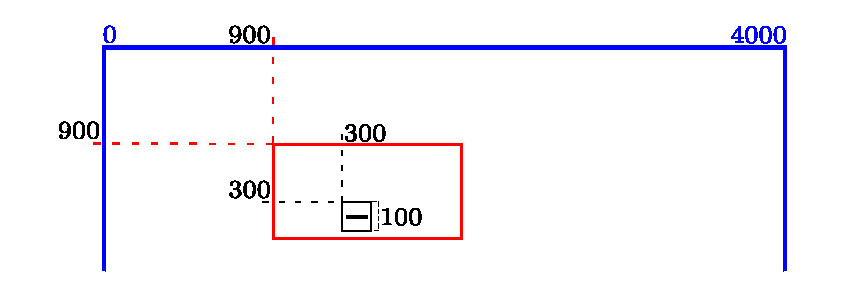
\includegraphics[width=0.75\textwidth]{../img/kap3_matice_umisteni.pdf}
	\caption{Příklad zobrazitelného prvku v~komponentě a~plátně \texttt{ContentCanvas}}
	\label{fig:matice_umisteni1}
\end{figure}
\begin{figure}[!bht]

\centering 
$\color{blue}
\begin{pmatrix} 
1 & 0 & 0 \\
0 & 1 & 0 \\
-900 & -900 & 1
\end{pmatrix}$
\color{black}
$\times$
\color{red} 
$\begin{pmatrix} 
1 & 0 & 0 \\
0 & 1 & 0 \\
1200 & 1200 & 1
\end{pmatrix}$
\color{black}
$=$
$\begin{pmatrix} 
1 & 0 & 0 \\
0 & 1 & 0 \\
300 & 300 & 1
\end{pmatrix}$
\caption{Výpočet \texttt{transform matrix} zobrazitelného prvku pomocí modré \texttt{transform matrix} plátna \texttt{ContentCanvas} a~červené \texttt{placement matrix}}
\end{figure}
\newpage
Podle \ref{spec:req:strategie2} chceme navíc zobrazení modifikovat rotací a~škálováním v~rámci strategií. Tyto transformace pak budou zaznamenány v~\texttt{placement matrix}. \linebreak K~násobení bychom mohli použít obecné maticové násobení implementované knihovnou SkiaSharp, které se ale provolává do C++ kódu knihovny Skia. Jelikož ale pracujeme pouze s~maticovými operacemi rotace, posunu a~škálování, můžeme násobit pouze některé prvky matic. Na následujícím fragmentu kódu je výsledná operace vytvářející \texttt{transform matrix} prvku, která zabere pouze šest násobení. 

\begin{csharpcode}
var canvasScaleX = canvasTransformMatrix[0]; 
var canvasScaleY = canvasTransformMatrix[4];
var canvasTransX = canvasTransformMatrix[2];
var canvasTransY = canvasTransformMatrix[5];

/* Other indices set to 0 */
var elementTransformMatrix = new SKMatrix { 
	/*A[3,3]*/ Persp2 = 1,
	/*A[1,1]*/ ScaleX = placementMatrix.ScaleX * canvasScaleX,
	/*A[1,2]*/ SkewY = placementMatrix.SkewY * canvasScaleY,
	/*A[2,1]*/ SkewX = placementMatrix.SkewX * canvasScaleX,
	/*A[2,2]*/ ScaleY = placementMatrix.ScaleY * canvasScaleY,
	/*A[3,1]*/ TransX = placementMatrix.TransX * canvasScaleX 
					    + canvasTransX,
	/*A[3,2]*/ TransY = placementMatrix.TransY * canvasScaleY 
						+ canvasTransY
};
\end{csharpcode}

Cyklus rozmístění zobrazitelného prvku bude muset pro výpočet matice \linebreak \texttt{placement matrix} prvku nastavit jeho umístění na \texttt{ContentCanvas} a~jeho hodnoty škálování a~rotace při transformaci strategií.

\subsubsection*{Vliv strategií na cyklus rozmístění}
Podle požadavku \ref{spec:zobrazitelne_prvky2} chceme zobrazitelné prvky strategiemi transformovat operacemi škálování a~rotace. Transformace může mít dopad pouze na vykreslení prvku nebo může změnit i~jeho velikost. Operace škálování by například mohla prvku proporcionálně přidělit jinou velikost a~prvek by na změnu reagoval. Měnila by se tak i~velikost plátna pro prvek a~zároveň s~ní i~umístění jeho kreslících příkazů. Taková implementace neodpovídá původnímu záměru prvky vykreslovat pokud možno nezávisle na zobrazení. Proto jsme se rozhodli transformace implementovat tak, aby strategie prvky pouze vizuálně transformovaly pomocí \texttt{placement matrix}. Během transformací se ale mění i~umístění prvků, pokud má prvek potomky. Cyklus rozmístění pak bude muset pro celý strom prvků při rotaci přepočítat umístění prvků a~jejich hodnoty pro výpočet \texttt{placement matrix}.

\subsubsection*{Umístění prvků na plátně}
\label{kap3:element_hit_test}
Podle \ref{spec:req:hit-test1} chceme dokázat zjistit, zda se nějaký bod plátna \texttt{ContentCanvas} nachází v~zobrazitelném prvku umístěném na tomto plátně. Jelikož můžou být prvky transformovány rotací a~škálováním, určení, zda se bod v~prvku nachází, může představovat složitý problém. Prvek umístěný v~plátně můžeme reprezentovat jako obdélník. K~jeho určení potřebujeme znát umístění, rotaci a~škálování prvku. Podle předchozí části dokážeme vytvořit \texttt{placement} \texttt{matrix}, která v~sobě nese tyto transformace. Pomocí této matice reprezentové \texttt{SKMatrix} dokážeme metodou \texttt{MapPoint()} levý horní vrchol obdélníku [0,0] nebo dolní pravý vrchol odpovídající velikosti prvku přetransformovat na body v~plátně \texttt{ContentCanvas}.

Tyto body by pak tvořily přímky popisující obdélník na plátně. Každá přímka určuje polorovinu, v~které se nachází obsah obdélníku, jako na obrázku \ref{fig:hit-test-polorovina}.

\begin{figure}[!bht]
	\centering
	
\includegraphics[width=\textwidth]{../img/kap3_rectangle_line_segment}
	\caption{Polorovina určená hranou obdélníku}
	\label{fig:hit-test-polorovina}
\end{figure}

Pokud se prvek nachází ve všech čtyřech polorovinách, je součástí obdélníku. Aby se pokaždé složitě neporovnávalo umístění přes poloroviny, můžeme vytvořit obdélník, který nazveme \texttt{bounding rectangle} a~bude ohraničovat vrcholy původního obdélníku, jako na obrázku \ref{fig:bounding-rectangle}, kde je zobrazen \texttt{bounding rectangle} prvku transformovaného rotací.

\begin{figure}[!bht]
	\centering
	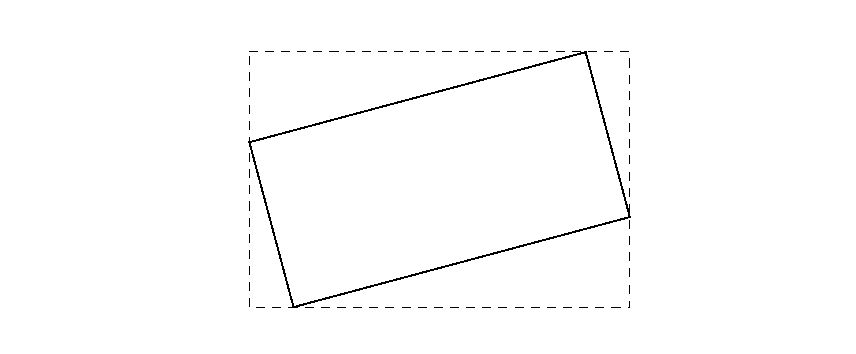
\includegraphics[width=\textwidth]{../img/kap3_rectangle_bounding}
	\caption{Čárkovaný \texttt{bounding rectangle} zobrazitelného prvku}
	\label{fig:bounding-rectangle}
\end{figure}

Rozhodli jsme se, že hit-testing bude na prvcích transformovaných rotací implementován tak, že se bod nejdříve porovná s~\texttt{bounding rectangle} a~v~případě úspěchu se provede přesné porovnání pomocí polorovin. V~případě prvků netransformovaných rotací stačí k~přesnému porovnání  použít pouze \texttt{bounding rectangle}. \texttt{Bounding rectangle} by bylo možné použít i~k~určení, zda se prvek nachází v~komponentě (\ref{kap3:view_element_bounding_check}) -- \texttt{bounding rectangle} by odpovídal červeným obdélníkům na plátně na obrázku \ref{fig:prvky_mimo_komponentu}. V~případě transformace rotací zabírá \texttt{bounding rectangle} o~něco více prostoru než je skutečná velikost prvku, ale jeho porovnání je rychlejší než přesné porovnání pomocí polorovin. Odhad, který používáme, v~nejhorších případech způsobí vykreslení velmi malého počtu prvků navíc.

\subsubsection*{Implementace zobrazitelných prvků}
\label{kap3:layout_cycle_view_element}
Implementaci zobrazitelných prvků bychom mohli reprezentovat rozhraním s~informacemi, které jsme si v~předchozích částech této podkapitoly uvedli. Toto rozhraní označíme jako \texttt{IViewElement}. Výhodou rozhraní by bylo, že~vývojář může implementovat vlastní cyklus rozmístění~z~\ref{spec:zobrazitelne_prvky2} podle konkrétního prvku metodami mimo rozhraní, odpovídající potřebám jeho implementace. Pokud \linebreak bychom například měli zobrazitelný prvek, který by představoval dopravní bod s~několika kolejemi, v~metodě umisťující prvek na plátno se nastaví, jestli má horizontální čáry jako koleje seskupit kvůli nedostatku prostoru na plátně do jedné čáry nebo je má vykreslit pro větší přehlednost vedle sebe.

Komplikací je, že pro implementaci rozhraní vývojář musí vypočítat přesné umístění prvků na~plátně \texttt{ContentCanvas}. V~případě práce se stromem prvků popisující obsah nákresného jízdního řádu podle \ref{spec:zobrazitelne_prvky1} by vývojář spíše preferoval možnost potomky prvku umístit v~rámci jeho souřadnic. Převod do souřadnic plátna \texttt{ContentCanvas} by se tak prováděl jen kvůli knihovně.

Další komplikací je aplikování strategií na prvky implementující toto rozhraní. Pokud bychom strom prvků přemístili nebo ho transformovali škálováním a~rotací, musí se změnit hodnoty pro výpočet \texttt{placement matrix} všech jeho prvků. Tento problém by musely řešit strategie úpravou hodnot rozhraní nebo by \texttt{IViewElement} mohlo obsahovat metody jako \texttt{Scale()} nebo \texttt{Rotate()}, které by strategie volaly a~úpravu stromu prvků by implementoval vývojář. V~předchozí části věnující se vlivu aplikování strategií na cyklus rozmístění jsme si ale uvedli, že by tyto operace měly implementaci prvku vývojářem ovlivnit co nejméně.

Informace rozhraní \texttt{IViewElement} se převádí na různé struktury jako \linebreak \texttt{placement matrix} nebo \texttt{bounding rectangle}. Všechny tyto převody by se odehrávaly během vykreslování, které ale nechceme zbytečně zpomalovat. Bylo by vhodnější, kdyby se už tyto struktury předpočítaly během cyklu rozmístění. Mohli bychom vytvořit základní implementaci zobrazitelných prvků, která implementuje nějaký obecný cyklus rozmístění, předpočítá tyto hodnoty a~umožní prvky umístit i~v~souřadnicích plátna rodičovského prvku.

Jelikož jsme určili, že by bylo vhodné, aby cyklus rozmístění produkoval další informace nebo struktury používané knihovnou, rozhodli jsme se, že jejich správné vytvoření zajistíme v~obecné implementaci, kterou dále budeme hledat. Vývojář bude v~potomcích základní implementace pouze přidávat konkrétní vlastnosti prvku -- vykreslení, určení požadované velikosti a~rozmístění obsahu na základě přiřazení konečné velikosti. Vývojáři tak obdrží hotovou implementaci, která bude vytvářet části důležité pro funkcionalitu knihovny.

\subsubsection*{Obecná implementace cyklu rozmístění zobrazitelných prvků}
Obecný cyklus rozmístění prvků musí být dostatečně konfigurovatelný pro různé scénáře. Podle \ref{spec:zobrazitelne_prvky2} například chceme změřit velikost prvku a~na základě této velikosti mu přiřadit jeho konečnou velikost. Konečná velikost prvku bude určovat velikost plátna pro vykreslení, ale i~hit-testovanou oblast nebo \texttt{bounding rectangle}. S~konečnou velikostí také budou pracovat strategie. Pokud by prvek tuto velikost přesáhl, nástroje by s~prvkem nemohly správně pracovat. Protože vytváříme nějakou obecnou implementaci pro knihovnu, chceme, aby špatné nastavení cyklu rozmístění bylo nějak deterministicky vyřešeno. Jelikož s~konečnou velikostí prvku pracuje mnoho částí knihovny, rozhodli jsme se, že pokud velikost prvku přesáhne přidělenou velikost, nebude rozmístěn. Problém s~rozmístěním se tak projeví hned a~ne při práci knihovny s~prvkem. Nechceme vyhovazovat výjimky, protože vytváříme obecnou implementaci a~některé aplikace pouze příliš velký prvek v~některých konfiguracích komponenty nezobrazí. Vývojáři umožníme ale implementaci rozšířit a~chybové stavy řešit i~jiným způsobem.

Podobný problém, na který jsme narazili, řeší i~GUI frameworky. Ty vytváří základní implementaci cyklu rozmístění pro jejich prvky uživatelského rozhraní. Frameworky pak pomocí hierarchie tříd cyklus rozmístění dále rozšiřují konfigurací jeho základní implementace. Toto řešení je vhodné i~pro naší knihovnu. Nemuseli bychom tak vymýšlet nové řešení, ale mohli bychom nějaké převzít a~upravit ho. Rozhodli jsme se proto použít nějakou existující implementaci a~přizpůsobit ji navíc požadavkům naší knihovny. Implementace se mezi různými frameworky zásadně neliší a~proto jsme se rozhodli vybrat k~implementaci cyklus rozmístění frameworku WPF, který se skládá z~\textit{measure} a~\textit{arrange} průchodů znázorněných na obrázku \ref{fig:arrange_WPF}:

\begin{figure}[!bht]
	\centering
	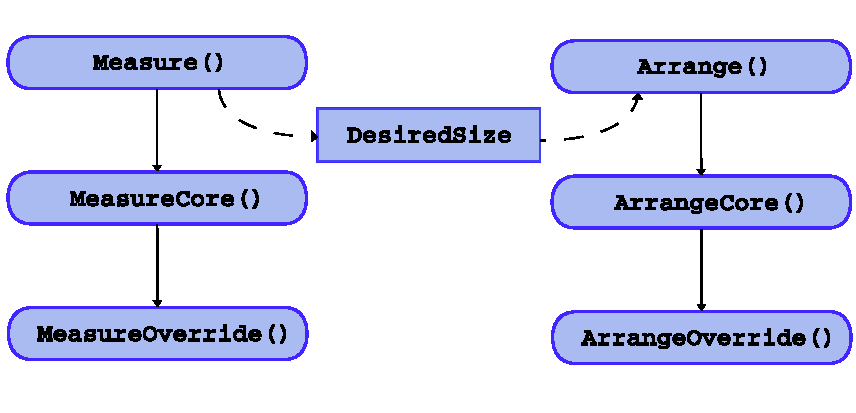
\includegraphics[width=\textwidth]{../img/kap3_wpf_element_layout_cycle_diagram}
	\caption{Schéma cyklu rozmístění pro prvek GUI frameworku WPF}
	\label{fig:arrange_WPF}
\end{figure}

Prvkům je možné nastavit vlastnosti jako \texttt{Margin}, \texttt{MinWidth}, \texttt{MaxWidth}, \linebreak \texttt{MinHeight}, \texttt{MaxHeight}. V~measure průchodu začínající metodou \texttt{Measure()} \linebreak nejdříve zjistíme velikost prvku. Velikost je v~rámci hierarchie volání získána nejdříve z~metody \texttt{MeasureOverride()}, kterou přetěžuje vývojář pro konkrétní implementaci prvku. Tato velikost je předána \texttt{MeasureCore()}, která v~základní implementaci ověřuje správnost vrácené hodnoty například vůči nastavení \linebreak \texttt{MaxWidth}, \texttt{MinWidth} a~případně ji upravuje. Vývojář může metodu přetížit za podobným účelem. Ověřená hodnota je předána \texttt{Measure()}, která ji přiřadí do vlastnosti \texttt{DesiredSize}. V~arrange průchodu je metodě \texttt{Arrange()} předána konečná velikost prvku. Metody \texttt{ArrangeOverride()} a~\texttt{ArrangeCore()} se chovají podobným způsobem jako jejich ekvivalenty v~measure průchodu. Cyklus rozmístění WPF vytváří mezi prvky explicitní vztahy, aby například invalidování potomka mohlo notifikovat o~změně rodiče, který by mohl změnu velikosti potomka vyřešit v~jemu přiřazené velikosti, případně by se notifikace šířila do jeho rodiče. Jelikož k~těmto situacím docházet při práci se zobrazitelnými prvky nebude, pro jednoduchost jsme se rozhodli explicitní vazby mezi prvky nevytvářet. Na potomky se volá pouze z~rodičovských prvků \texttt{Arrange()} a~\texttt{Measure()}.

\subsubsection*{Výpočet struktur používaných knihovnou v~cyklu rozmístění}
\label{kap3:upravy_zobrazitelnych_prvku_strategiemi}
Určili jsme, že v~základní implementaci cyklu rozmístění spočítáme hodnoty jako \texttt{placement matrix} nebo \texttt{bounding rectangle}. Navíc podle \ref{spec:req:strategie2} chceme, aby zobrazení prvků bylo možné upravovat rotací a~škálováním a~prvek přerozmístit. Všechny tyto úpravy je možné zahrnout do \texttt{placement matrix}. Při vykonávání těchto modifikací prvku chceme, aby byly aplikovány na všechny jeho potomky.

Jelikož se výpočet těchto hodnot bude aplikovat i~pomocí metod, kterými strategie prvek transformují a~je celkem náročné ho implementovat, chtěli bychom najít nějakou jednu metodu, v~které by se výpočet provedl. Pokud se podíváme, jak transformace souvisí s~cyklem rozmístění, strategie nejdříve musí zjistit velikost prvku, přiřadit mu konečnou velikost a~pak ho případně transformovat rotací nebo škálováním. Metoda \texttt{Arrange()}, která by prvku přiřadila konečnou velikost, by mohla získat v~rámci jejího volání \texttt{placement matrix}. Konfigurace \texttt{placement matrix} by pak mohly být následující:

\begin{enumerate}
	\item	Aplikováním \texttt{placement matrix} rodičovského prvku můžeme prvek \newline\texttt{Arrange()} umístit v~souřadnicích rodičovského prvku
	\item	Aplikováním \texttt{placement matrix} jako identity můžeme prvek \texttt{Arrange()} umístit v~souřadnicích \texttt{ContentCanvas}
	\item	Aplikováním rotace nebo škálování na \texttt{placement matrix} můžeme vytvářet transformace rotace a~škálování strategiemi
\end{enumerate}
 
Měli bychom tedy nějakou interní metodu \texttt{ArrangeInternal()}, která by přijímala různé \texttt{placement matrix}. Vývojáři by volali na zobrazitelném prvku \linebreak \texttt{Arrange()}, \texttt{Scale()}, \texttt{Rotate()} a~\texttt{Reposition()}. Tyto metody upraví \texttt{placement matrix} a~předají jí \texttt{ArrangeInternal()} metodě. Pokud se zavolá \linebreak v~\texttt{ArrangeOverride()} na potomka \texttt{Arrange()}, předá se mu upravená \texttt{placement matrix} a~stejný výpočet probíhá znovu v~potomku. Pomocí \texttt{placement matrix} se pak vypočítá \texttt{bounding rectangle} i~ostatní hodnoty související s~transformací. Ačkoliv cyklus rozmístění tak probíhá pro každou tuto operaci znovu, rozhodli jsme se tento přístup použít, protože neduplikuje kód a~aplikování operace znovu nepředstavuje velké výkonnostní omezení, jelikož transformace strategiemi neprobíhají na větších stromech prvků a~vyskytují se v~cyklu rozmístění, ke kterému při běhu aplikace nedochází často.

\newpage
\subsection{Kreslení po vrstvách}
\label{kap3:drawing_layers}
Podle podkapitoly \ref{kap2:drawing_layers} chceme umožnit obsah vykreslovat ve vrstvách. Ve zmíněné podkapitole jsme uvedli příklad, kdy chceme do nové vrstvy v~popředí vynést vybraný vlak z~vrstvy vykreslující všechny vlaky. Zásadní problém, kterému se budeme snažit předejít, je vykreslení stejného obsahu ve více vrstvách opakovaně -- vybraný vlak by se vykreslil v~nové i~původní vrstvě. Všechny vlaky se nachází v~nějakém seznamu a~v~původní vrstvě se vykreslí následovně:

\begin{csharpcode}
foreach(var train in Trains) {
	drawingCanvas.Draw(train);
}
\end{csharpcode}

Mohli bychom vybraný vlak umisťovaný do nové vrstvy z~\texttt{Trains} odebrat. Tímto ale zasahujeme do modelu aplikace, při operaci, která svým významem model nemění -- vybraný vlak se pouze přenáší do popředí. Další možností by bylo vytvořit nový seznam, který obsahuje prvky nacházejí se ve vrstvě nebo každému zobrazovanému vlaku přidat informaci, zda je ho možné ve vrstvě vykreslit. Zásadním problémem obou těchto řešení je fakt, že zasahují do implementace obsahu v~původní vrstvě:

\begin{csharpcode}
foreach(var train in Trains) {
	if (currentLayer.Contains(train)) {
		drawingCanvas.Draw(train);	
	}	
}
\end{csharpcode}

Problém můžeme řešit na úrovni knihovny tak, aby tato implementace nebyla změněna. Prvky jako vlak by implementovaly rozhraní \texttt{IVisual}, které bude nést informaci o~přidělené vrstvě prvku. \texttt{DrawingCanvas} bude vědět, jakou vrstvu vykresluje. Pokud budeme chtít \texttt{IVisual} na plátno vykreslit, nejdříve se provede porovnání vrstev a~pokud jsou stejné, prvek se vykreslí. Jediná nevýhoda je, že se vrstva musí přenastavit všem prvkům stromu reprezentující vybraný vlak, aby se po porovnání vykreslily.

Jelikož jsme v~požadavku \ref{spec:zobrazitelne_prvky1} určili, že obsah nákresného jízdního řádu bude systematicky popsatelný různými prvky, rozhodli jsme se, že prvky budou implementovat rozhraní jako \texttt{IVisual} a~\texttt{DrawingCanvas} ověří jejich vykreslení. \texttt{IVisual} bude implementováno v~nějaké základní třídě všech vykreslitelných prvků, která je předkem \texttt{ViewElement}. V~knihovně tak vytváříme mechanismus, který vývojář může používat a~nevytvářet vlastní řešení. Zmíněnou nevýhodu v~další části odstraníme a~ještě řešení vylepšíme.

\pagebreak
\subsubsection*{Konfigurace vrstev}
V~dosavadní představě si v rozhraní \texttt{IVisual} uchováváme pouze vrstvu, \linebreak v~které se prvek nachází. Když vývojář změní prvku vrstvu, musí si pamatovat, v~jaké předchozí vrstvě se prvek nacházel. Proces přemisťování prvků mezi vrstvami probíhá tak, že vývojář vrstvu změní a~pak ji zase nahradí původní. V~příkladu prvků vlaku vyneseného do popředí se jeho prvky nejdříve při inicializaci obsahu přiřadí do vrstvy všech vlaků a~při výběru vlaku se přenesou do vrstvy popředí. Pak se případně vrací do vrstvy původní. Proces přiřazování a~odebírání vrstev tak odpovídá práci se zásobníkem. Aby si vývojář nemusel pamatovat, v~jaké původní vrstvě se prvek nacházel, tento zásobník každému z~prvků přidáme.

Nevýhodou současného řešení je potřeba nastavovat vrstvu všem prvkům, které bychom chtěli vykreslit. Tuto nevýhodu bychom mohli na základě následujícího pozorování odstranit. Předpokládejme, že v~počátečním stavu aplikace problém, kdy by se jeden prvek vykreslil ve více vrstvách zároveň, nenastává. Chtěli bychom nalézt řešení, jak nastavování vrstev v~počátečním stavu přeskočit. Vytvoříme vrstvu, kterou nazveme jako \texttt{default layer}. Pokud ji má prvek nastavenou, kontrola vrstvy se před vykreslením nevykoná. Jelikož pracujeme se zásobníkem, bude tato vrstva umístěna na spodku zásobníku, jako počáteční stav. Pokud použijeme příklad s~vybraným vlakem, při jeho přesunu do nové vrstvy bychom už vrstvu změnili všem jeho prvkům.

\subsection{Implementace hit-testingu}
\label{kap3:hit_test_tree}
V~části \ref{kap3:element_hit_test} jsme určili, jak probíhá hit-testování na každém zobrazitelném prvku. Nyní si vysvětlíme, jak podle požadavku \ref{spec:req:hit-test2} implementujeme průchod zobrazitelných prvků obsahu nákresného jízdního řádu a~získáme z~něj ty, které v~hit-testování uspěly. Tyto prvky bude chtít vývojář získat podle pořadí jejich vykreslení, s~tím, že většinou bude pracovat s~prvkem, který je vykreslován v~popředí a~překrývá tak ostatní prvky, které v~hit-testu také uspěly. 

Průchod prvků by mohl implementovat sám vývojář. Postupně by procházel všechny prvky, tvořící dohromady stromovou strukturu. V~některých prvcích stromu by ale mohl narazit na problém. V~příkladu uvedeném v~\ref{kap3:drawing_layers} máme zobrazitelný prvek vykreslující všechny vlaky v~seznamu \texttt{Trains}. Vývojář by tento seznam prošel a~každý prvek vlaku ověřil v~hit-testu. Podle \ref{kap3:drawing_layers} se ale vlaky můžou nacházet v~různých vrstvách, čili by sekvenční průchod seznamu případně neposkytl správné pořadí vykreslení a~při průchodu prvků ve více vrstvách by se konkrétní prvek mohl vyskytnout v~úspěšně otestovaných prvcích vícekrát.

Průchod stromu prvků jsme se proto rozhodli implementovat v~knihovně. Otestování celého obsahu odpovídá průchodu stromem, kdy otestujeme obsah rozdělený do vrstev, vykreslovaných podle jejich pořadí. Každá vrstva bude obsahovat prvek, který bude kořenem jejího obsahu. K~rozhraní \texttt{IVisual} z~\ref{kap3:drawing_layers} bychom přidali metodu \texttt{HitTest()}, hit-testující vizuální prvek vůči nějakému bodu a~metodou poskytující potomky k~hit-testování \texttt{ProvideChildrenToHitTest()}. Z~této metody se pak vyberou jen ty prvky, které se nachází ve stejné vrstvě jako rodičovský prvek. Musíme ještě určit pořadí, v~kterém bude knihovna poskytovat úspěšně otestované prvky. Metodu \texttt{ProvideChildrenToHitTest()} bychom chtěli nechat vývojáře implementovat tak, aby prvky poskytovala v~pořadí vykreslení:

\begin{csharpcode}
public void OnDraw(DrawingCanvas drawingCanvas) {
	foreach(var train in Trains) {
		drawingCanvas.Draw(train);	
	}
}

public IEnumerable<IVisual> ProvideChildrenToHitTest() {
	foreach(var train in Trains) {
		yield return;
	}
}
\end{csharpcode}

To ale znamená, že první poskytnutý prvek je ten, který se vykreslí na spodku. Vývojář by mohl projít seznam v~opačném pořadí, to ale představuje komplikaci v~implementaci rozhraní. Úspěšně otestované prvky bychom při průchodu stromem mohli uchovávat v~nějakém seznamu, odpovídající pořadí vykreslení. Jelikož úspěšně testovaných prvků je malé množství, rozhodli jsme se, že vývojář v~rozhraní poskytne prvky podle pořadí vykreslení. Průchod tedy bude implementován tak, že se postupně navštíví všechny vrstvy s~jejich obsahem podle pořadí vykreslení. Pokud chceme prvek, který překrývá ostatní, najdeme ho na konci tohoto seznamu. Proto bychom si místo seznamu mohli pamatovat jen jeden prvek, který se vykreslí jako poslední. Bylo by možné místo pevného seznamu použít jinou implementaci průchodu, kterou si nyní představíme.

Průchod stromu prvků pro hit-testování řeší i~uživatelská rozhraní. Například GUI framework WPF implementuje obecný průchod stromem, kdy se při navštívení prvku zavolá vývojářem dodaná metoda delegáta \texttt{HitTestFilterCallback}, v~které může vývojář podle prvku rozhodnout, jak má dále průchod stromem pokračovat. Průchodu stromem se dále předává metoda delegáta \linebreak \texttt{HitTestResultCallback}, která se volá, pokud byl prvek vůči hit-testingu \linebreak úspěšný. Také určí, jak při průchodu stromem pokračovat. V~základním nastavení je tato implementace lehká na konfiguraci -- v~\texttt{HitTestResultCallback} by se úspěšně testované prvky přidávaly do seznamu, který jsme chtěli v~původní implementaci použít.
Vývojář může průchod stromem urychlit, jelikož dodání implementace delegáta \texttt{HitTestFilterCallback} umožňuje přeskočit všechny prvky v~nějakém podstromu, u~kterých víme, že se s~nimi pracovat nebude. Jelikož implementace odpovídá našim potřebám a~můžeme převzít funkční kód doplněný o~potencionálně využitelná rozšíření, rozhodli jsme se ji použít.

\newpage
\subsection{Implementace strategií}
\label{kap3:implementace}
Pro splnění požadavku \ref{spec:zobrazitelne_prvky1} musíme najít nástroje, které umožní systematicky popsat proces implementace strategií. Rozhodli jsme se, že tento proces rozdělíme do částí, kde každá část má jednu zodpovědnost\footnote{Single responsibility principle~\cite{Martin:2003:ASD:515230}}. Tyto částí si nyní popíšeme a~zdůvodníme jejich používání.

\subsubsection*{Segmenty strategií}
Strategiím je potřeba vyhradit nějaký vodorovný pruh, do kterého můžou umístit zobrazitelné prvky. Tyto pruhy označíme jako \textit{segmenty}. Umístění i~výšku segmentu vývojář určí v~cyklu rozmístění před samotným aplikováním strategie, jelikož jsou segmenty součástí zobrazitelných prvků popisujících nákresný jízdní řád, jako třeba místa pro umisťování kót kolem horizontálních čar dopravních bodů. Nechceme, aby vývojář vytvářel ve svém modelu vlastní struktury, které by segmenty určovaly. Nemůžeme pak jejich konkrétní implementaci zapojit do nástrojů pracujících se strategiemi a~navíc představují další část pro vývojáře, kterou musí implementovat. Ke strategii pro rozmisťování kót do ostrých úhlů bychom potřebovali dva segmenty kolem dopravních bodů, jako na obrázku \ref{fig:segments_upper_lower}. Segmenty v~příkladu je možné rozlišit -- podle dopravního bodu a~dolního nebo horního umístění. Proto pro segment zavedeme identifikaci označovanou jako \texttt{SegmentType}, která umožní segmenty kategorizovat. Segmenty patřící pod jeden typ bude spravovat registr \texttt{SegmentRegistry}, který bude přijímat registrace segmentů a~poskytovat segmenty podle \texttt{SegmentType}, čehož můžou využít další nástroje pracující se strategiemi.

\begin{figure}[!bth]
	\centering
	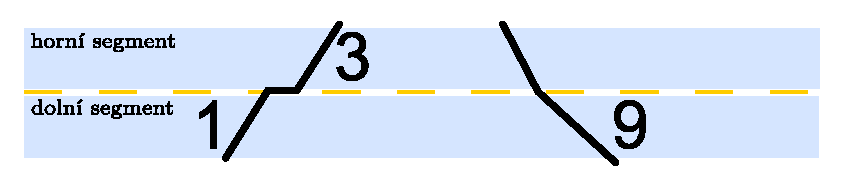
\includegraphics[width=\textwidth]{../img/kap3_segment_upper_lower}
	\caption{Horní a~dolní segment dopravního bodu pro umístění kót}
	\label{fig:segments_upper_lower}
\end{figure}

\subsubsection*{Zařazení zobrazitelných prvků do strategií}
\label{kap4:strategy_placement_type}
Když chce vývojář přidat do strategie zobrazitelný prvek, musí se zjistit, do jakého \texttt{SegmentType} prvek patří. Pokud by vývojář přidával prvek přímo do segmentu, musel by sám určit \texttt{SegmentType}. To ale může představovat problém. Uvažme případ, kdy chceme přidat odjezdovou kótu z~nějakého dopravního bodu, jako na obrázku \ref{fig:view_element_strategy_registration}. \texttt{SegmentType} je závislý na směru jízdy vlaku, čili vývojář musí sám složitě podle výpočtu zjistit, kam prvek podle směru patří. Vývojář by mohl při přidání prvku uvést jiný typ, přirozenější pro specifikaci umístění, označovaný jako \texttt{PlacementType}, který se na \texttt{SegmentType} převede. Vývojář by při přidání prvku uvedl informaci v~\texttt{PlacementType} 
\includegraphics[height=10.0pt]{../img/cas_osa_typ_1} se směrem (příjezd nebo odjezd). Bude pak existovat rozhraní \texttt{ITypeConverter}, které převede tuto informaci na \texttt{SegmentType} 
\includegraphics[height=10.0pt]{../img/cas_osa_typ_2} (lower, upper). Rozhodli jsme se tyto dva typy s~rozhraním pro převod zavést.

\begin{figure}[!bth]
	\centering
	
\includegraphics[width=\textwidth]{../img/kap3_view_element_segment_registration}
	\caption{Přidání kóty odjezdu do strategie}
	\label{fig:view_element_strategy_registration}
\end{figure}

\subsubsection*{Spravování zobrazitelných prvků v~strategiích}
Vývojář bude přidávat prvky do strategie pomocí nástroje \texttt{StrategyManager} uvedením \texttt{PlacementType}. \texttt{StrategyManager} 
zajišťuje přiřazení prvků do správných segmentů a~strategií. Vývojář tak nemusí přímo pracovat s~jejich konkrétními implementacemi. Existují situace, kdy je nutné invalidovat všechny přidané zobrazitelné prvky -- například, když se odstraňuje vlak nebo se jeho trasa zcela mění. Pro každý logický celek prvků, který má omezenou dobu existence (\textit{scope}), bude vytvořen nový \texttt{StrategyManager}, zajišťující odstranění prvků ze struktur strategií nebo segmentů -- zabraňujeme tak \textit{memory leakům}, kdy by tyto struktury držely jedinou referenci na prvek jinak již neexistující části obsahu, jelikož je vývojář zapomněl odebrat.

\subsubsection*{Dockery zobrazitelných prvků}
\textit{Docker} implementuje vhodné rozmístění zobrazitelných prvků. V~cyklu rozmístění obdrží od \texttt{StrategyManager} všechny přidané prvky a~umístí je do oblastí segmentů. Implementace dockeru může vypadat tak, že nejdříve prvek změří, přidělí mu požadovanou velikost přes \texttt{Arrange()} a~pak na něj podle \texttt{SegmentType} a~dalších parametrů aplikuje správnou metodu, která ho podle \ref{spec:req:strategie2} transformuje a~umístí. Docker je takto možné v~aplikaci vyměnit a~reimplementovat, jelikož přímo není propojený s~nástroji pro strategii.